\newcommand{\nom}{Porte conteneur}
\newcommand{\sequence}{03}
\newcommand{\num}{04}
\newcommand{\type}{TD}
\newcommand{\descrip}{Résolution d'un problème en utilisant des méthodes algorithmiques}
\newcommand{\competences}{Alt-C3: Concevoir un algorithme répondant à un problème précisément posé}
\documentclass[10pt,a4paper]{article}
  \usepackage[french]{babel}
  \usepackage[utf8]{inputenc}
  \usepackage[T1]{fontenc}
  \usepackage{xcolor}
  \usepackage[]{graphicx}
  \usepackage{makeidx}
  \usepackage{textcomp}
  \usepackage{amsmath}
  \usepackage{amssymb}
  \usepackage{stmaryrd}
  \usepackage{fancyhdr}
  \usepackage{lettrine}
  \usepackage{calc}
  \usepackage{boxedminipage}
  \usepackage[french,onelanguage, boxruled,linesnumbered]{algorithm2e}
  \usepackage[colorlinks=false,pdftex]{hyperref}
  \usepackage{minted}
  \usepackage{url}
  \usepackage[locale=FR]{siunitx}
  \usepackage{multicol}
  \usepackage{tikz}
  \makeindex

  %\graphicspath{{../Images/}}

%  \renewcommand\listingscaption{Programme}

  %\renewcommand{\thechapter}{\Alph{chapter}}
  \renewcommand{\thesection}{\Roman{section}}
  %\newcommand{\inter}{\vspace{0.5cm}%
  %\noindent }
  %\newcommand{\unite}{\ \textrm}
  \newcommand{\ud}{\mathrm{d}}
  \newcommand{\vect}{\overrightarrow}
  %\newcommand{\ch}{\mathrm{ch}} % cosinus hyperbolique
  %\newcommand{\sh}{\mathrm{sh}} % sinus hyperbolique

  \textwidth 160mm
  \textheight 250mm
  \hoffset=-1.70cm
  \voffset=-1.5cm
  \parindent=0cm

  \pagestyle{fancy}
  \fancyhead[L]{\bfseries {\large PTSI -- Dorian}}
  \fancyhead[C]{\bfseries{{\type} \no \numero}}
  \fancyhead[R]{\bfseries{\large Informatique}}
  \fancyfoot[C]{\thepage}
  \fancyfoot[L]{\footnotesize R. Costadoat, C. Darreye}
  \fancyfoot[R]{\small \today}
  
  \definecolor{bg}{rgb}{0.9,0.9,0.9}
  
  
  % macro Juliette
  
\usepackage{comment}   
\usepackage{amsthm}  
\theoremstyle{definition}
\newtheorem{exercice}{Exercice}
\newtheorem*{rappel}{Rappel}
\newtheorem*{remark}{Remarque}
\newtheorem*{defn}{Définition}
\newtheorem*{ppe}{Propriété}
\newtheorem{solution}{Solution}

\newcounter{num_quest} \setcounter{num_quest}{0}
\newcounter{num_rep} \setcounter{num_rep}{0}
\newcounter{num_cor} \setcounter{num_cor}{0}

\newcommand{\question}[1]{\refstepcounter{num_quest}\par
~\ \\ \parbox[t][][t]{0.15\linewidth}{\textbf{Question \arabic{num_quest}}}\parbox[t][][t]{0.85\linewidth}{#1\label{q\the\value{num_quest}}}\par
~\ \\}

\newcommand{\reponse}[4][1]
{\noindent
\rule{\linewidth}{.5pt}\\
\textbf{Question\ifthenelse{#1>1}{s}{} \multido{}{#1}{%
\refstepcounter{num_rep}\ref{q\the\value{num_rep}} }:} ~\ \\
\ifdef{\public}{#3 ~\ \\ \feuilleDR{#2}}{#4}
}

\newcommand{\cor}
{\refstepcounter{num_cor}
\noindent
\rule{\linewidth}{.5pt}
\textbf{Question \arabic{num_cor}:} \\
}


\usepackage{enumitem}

\setenumerate[1]{align=left,label=\arabic*}
\setenumerate[2]{before=\stepcounter{enumi},label*=.\arabic*,leftmargin=1.2em,align=left}


\ifdef{\public}{\excludecomment{solution}}


\begin{document}

\begin{center}
{\Large\bf {\type} \no {\numero} -- \descrip}
\end{center}

\SetKw{KwFrom}{de} 

\begin{boxedminipage}{.9\textwidth} 
\begin{itemize}
 \item Faire tous les exercices dans un même fichier {NomPrenom.py} à sauvegarder,
 \item mettre en commentaire l'exercice et la question traités (ex: \# Exercice 1),
 \item ne pas oublier pas de commenter ce qui est fait dans votre code (ex: \# Je crée une fonction pour calculer la racine d'un nombre),
 \item il est possible de demander un déblocage pour une question, mais celle-ci sera notée 0,
 \item il faut vérifier avant de partir que le code peut s'exécuter et qu'il affiche les résultats que vous attendez.
\end{itemize}
\end{boxedminipage}

\section*{Générer la trajectoire d'une sonde de la Terre vers Mars}

\begin{figure}[ht!]
\begin{minipage}{0.48\linewidth}
Le 18 février 2021 à 20 h 44, la sonde Perseverance, partie de la Terre le 30 juillet 2020, a atterri sur Mars.

~\

Après avoir été propulsée par une fusée pour s'extraire de l'attraction terrestre, elle entre sur une orbite autour du Soleil le long de laquelle elle se rapproche progressivement de  l'orbite de Mars, jusqu'à l'intercepter.

~\

L'objectif de cette épreuve est de déterminer la trajectoire (simplifiée) de la sonde à partir de l'étude des orbites de la Terre et de Mars.
\end{minipage}\hfill
\begin{minipage}{0.47\linewidth}
  \begin{center}
  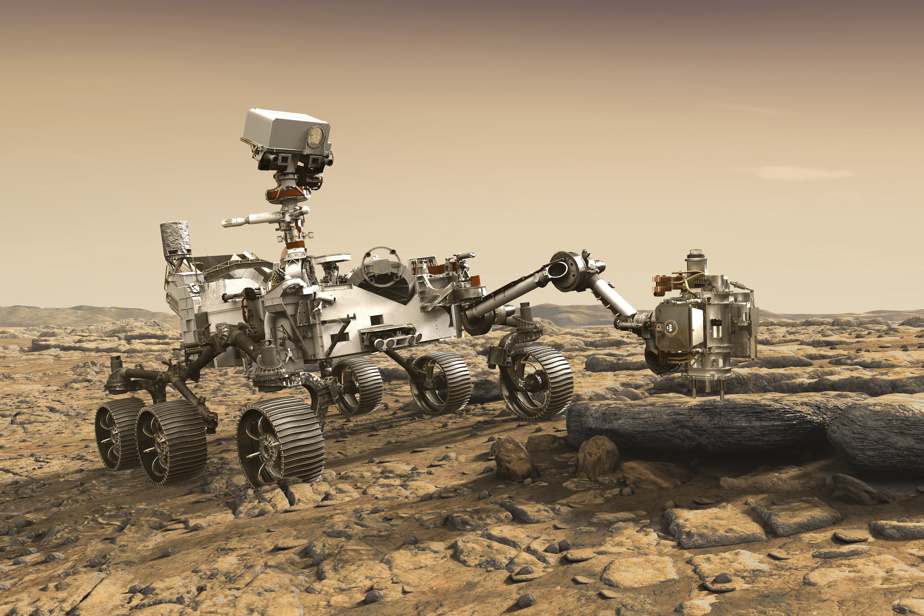
\includegraphics[width=0.9\linewidth]{img/perseverance}
  \caption{Image virtuelle du robot Perseverance sur Mars.}
  \label{perseverance}  \end{center}
 
\end{minipage}
\end{figure}

\section*{Tracé et découpage des trajectoires de la Terre et de Mars.}

\begin{figure}[ht!]
\begin{minipage}{0.48\linewidth}
Les paramètres (géométriques ou numériques) d'une ellipse utiles pour cette épreuve sont :
\begin{itemize}
 \item la longueur du grand rayon (ou demi-grand axe), notée $a$,
 \item la longueur du petit rayon (ou demi-petit axe), notée $b$,
 \item la distance séparant le centre de l'ellipse et un des foyers ($F$), notée $c$,
 \item l'excentricité de l’ellipse (strictement comprise entre 0 et 1), notée $e=\frac{c}{a}$,
\end{itemize}
\end{minipage}\hfill
\begin{minipage}{0.48\linewidth}
  \begin{center}
  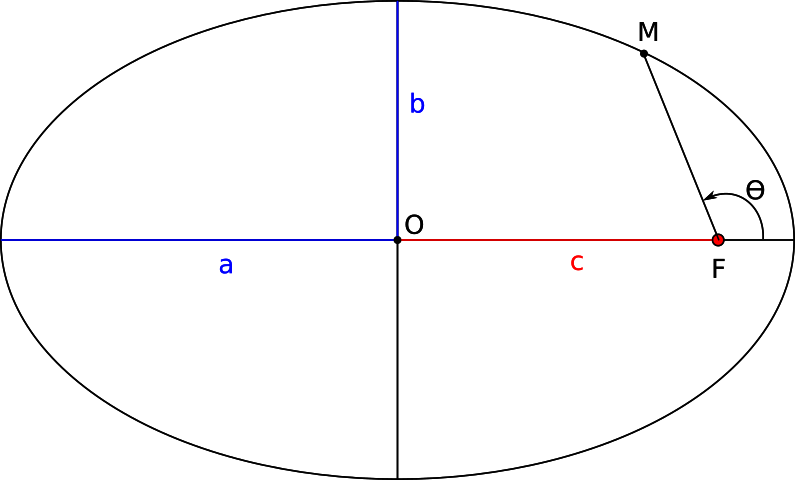
\includegraphics[width=0.9\linewidth]{img/ellipse}
  \caption{Représentation mathématique d'une ellipse.}
  \label{ellispe}
  \end{center} 
\end{minipage}
\end{figure}

\begin{enumerate}
\item  Mettre en en-tête du fichier les éléments suivants:
 \begin{itemize}
  \item \verb?import matplotlib.pyplot as plt?
  \item \verb?import numpy as np?
 \end{itemize}

~\

Soit $M$ un point de l'ellipse, le rayon $FM$ peut être calculé en fonction de l'angle $\theta$ en utilisant la formule suivante:

\begin{center}
$r(\theta)=\frac{a\cdot (1-e^2)}{1+e\cdot cos(\theta)}$
\end{center}

\item Écrire la fonction \verb?rayon(a,e,theta)? qui renvoie la valeur de $r(\theta)$.

\begin{solution}~\ \\
\begin{minted}{python}
def rayon(a,e,theta):
    return a*(1-e**2)/(1+e*np.cos(theta))
\end{minted}
\end{solution}
 
On donne pour la trajectoire de la Terre:
\begin{itemize}
\item $a_{terre}=\SI{1,49e11}{\meter}$ (\verb?aterre? dans le script),
\item $e_{terre}=0,016$ (\verb?eterre? dans le script),
\item La révolution s'effectuant autour du Soleil, le point $F$, sera appelé $S$ dans la suite.
\end{itemize}

Aide Python:
\begin{itemize}
 \item Il est possible sous Python de tracer une courbe en coordonnées polaires en utilisant la fonction \verb?plt.polar(theta,r)?,
 \item On générera les valeurs de $\theta$ à l'aide de la fonction \verb?theta=np.arange(0,2*np.pi,0.001)?.
\end{itemize}

\item Écrire le code permettant de tracer la trajectoire de la Terre et faire apparaître la figure \ref{fig01}.

\begin{figure}[!ht]
\centering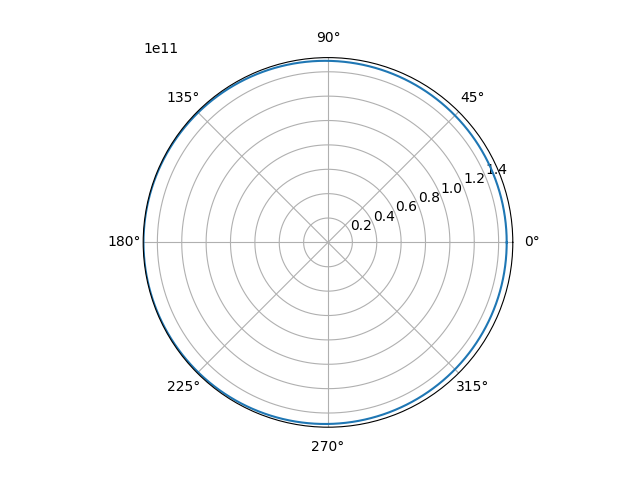
\includegraphics[width=0.6\linewidth]{img/Figure_1}
\caption{Tracé de la trajectoire de la Terre autour du Soleil sous Python.}
\label{fig01}
\end{figure}

\begin{solution}~\ \\
\begin{minted}{python}
aterre=1.49*10**11
eterre=0.016
theta=np.arange(0,2*np.pi,0.001)
plt.polar(theta,rayon(aterre,eterre,theta))
plt.show()
\end{minted}
\end{solution}
 
On peut calculer la période (en secondes) de révolution d'un astre autour du Soleil à l'aide de la loi de Kepler suivante:
$P=\sqrt{\frac{4\cdot a^3\cdot \pi^2}{G\cdot(m_{astre}+m_{soleil})}}$

On donne pour effectuer les calculs:
\begin{itemize}
 \item $G=\SI{6,67e-11}{\newton\meter\squared\per\kilo\gram\squared}$,
 \item $m_{soleil}=\SI{1,97e30}{\kilo\gram}$ (\verb?msoleil? dans le script),
 \item $m_{terre}=\SI{6e24}{\kilo\gram}$ (\verb?mterre? dans le script),
\end{itemize}

\item Créer une fonction \verb?periode(a,m)? qui renvoie la période de révolution (en jours) d'un astre de masse $m$ et de demi-grand axe $a$. Afficher le résultat numérique correspondant à celle de la Terre. Cette valeur était-elle prévisible ? (Donner la réponse à l'aide d'un \verb?print("Réponse: ")?).

\begin{solution}~\ \\
\begin{minted}{python}
G=6.67*10**(-11)
msoleil=1.97*10**30
mterre=6*10**24
def periode(a,m):
    P=np.sqrt(4*a**3*np.pi**2/(G*(mterre+msoleil)))
    return P/(3600*24)

P=periode(aterre,mterre)
print(P)
print("On trouve environ 365 jours soit une année, durée de révolution autour du soleil. Le résultat est donc cohérent.")
\end{minted}
\end{solution}

\subsection*{Deuxième loi de Kepler}

\begin{figure}[ht!]
\begin{minipage}{0.5\linewidth}
La deuxième loi de Kepler ou « loi des aires » dit que le rayon-vecteur reliant une planète au Soleil balaie des aires égales en des durées égales. Le rayon-vecteur est un segment reliant le Soleil, situé à un des foyers de l'ellipse, à la planète située sur l'ellipse.

~\


Cela signifie que sur la figure \ref{fig02}, l'astre, dont l'orbite est tracée en noir, mettra autant de temps pour passer du point $P_1$ au point $P_2$ que de $A_1$ à $A_2$, car les deux portions d'ellipse $SP_1P_2$ et $SA_1A_2$ ont la même aire.

\end{minipage}\hfill
\begin{minipage}{0.48\linewidth}
  \begin{center}
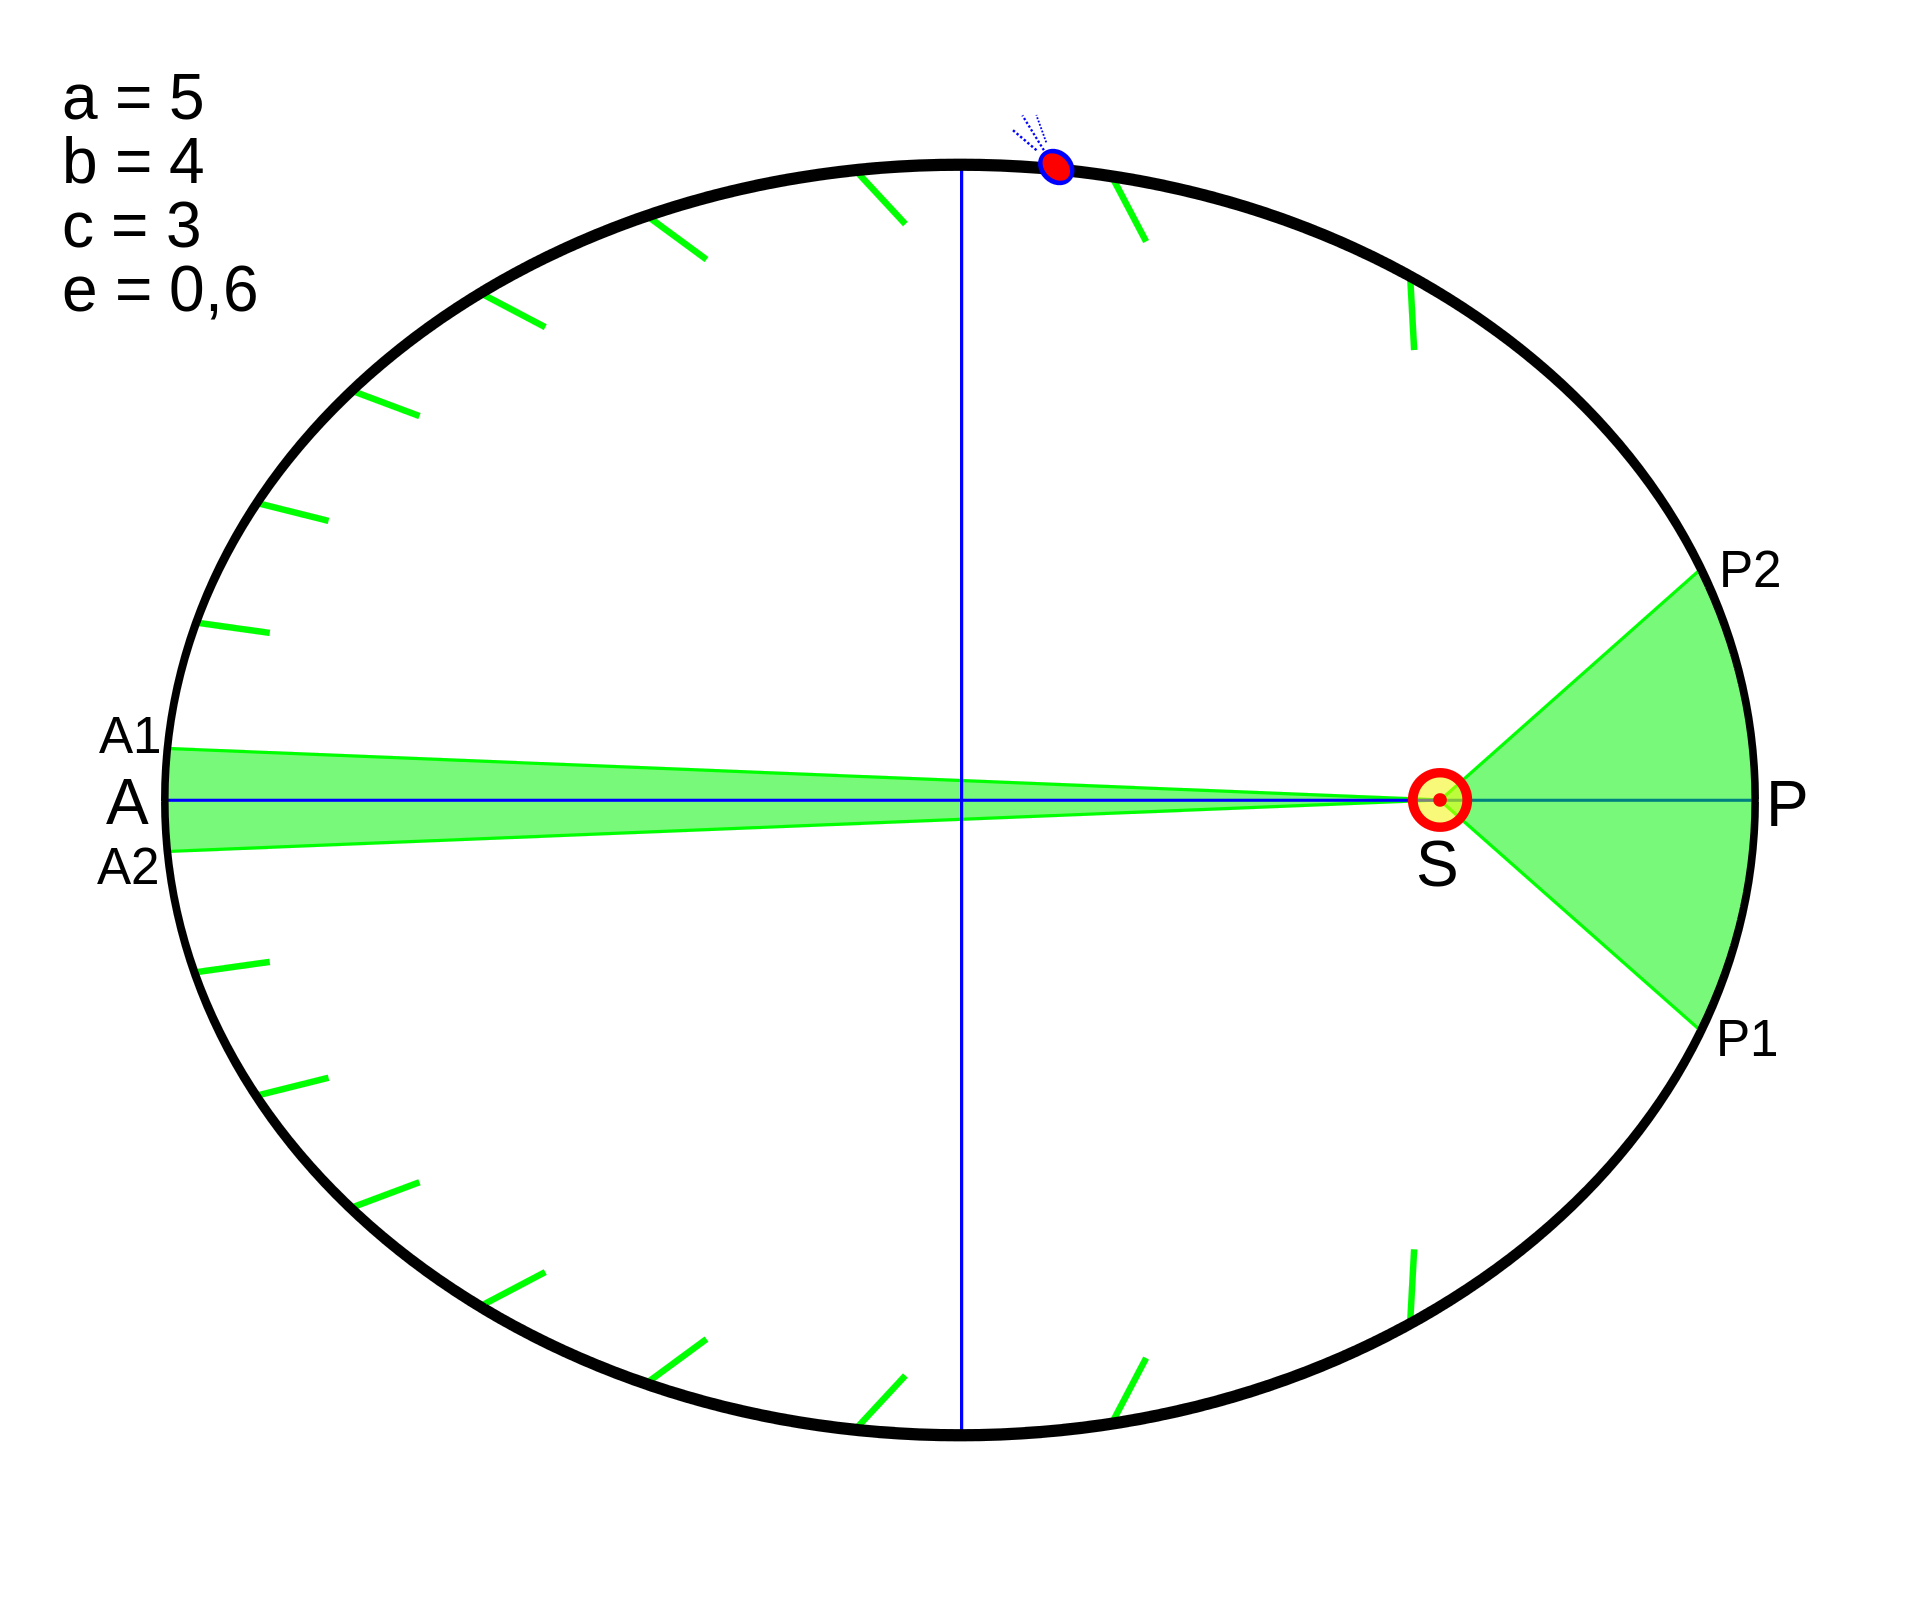
\includegraphics[width=0.9\linewidth]{img/kepler_2}
\caption{Construction illustrant la deuxième loi de Kepler.}
\label{fig02}
  \end{center} 
\end{minipage}
\end{figure}

Dans un premier temps, nous allons discrétiser la trajectoire en la décomposant en un ensemble de segments $M_iM_{i+1}$.

L'aire de la section d'ellipse $SM_iM_{i+1}$ est définie par la formule suivante:

$aire(i)=\frac{1}{2}\cdot r_{i+1}\cdot r_i\cdot \sin(\theta_{i+1}-\theta_i)$, avec ($\theta_i$,$r_i$) les coordonnées polaires du point $M_i$ par rapport à $S$.

\item Écrire la fonction \verb?calcul_aire(a,e,i)? qui renvoie l'aire de la section d'ellipse $SM_iM_{i+1}$ à partir des paramètres $a$ et $e$ de l'ellipse et de l'index $i$ du point $M_i$. Afficher l'aire de l'élément d'index $i=0$ de l'ellipse de trajectoire de la Terre.

\begin{solution}~\ \\
\begin{minted}{python}
def calcul_aire(a,e,i):
    return 0.5*rayon(a,e,theta[i+1])*rayon(a,e,theta[i])*np.sin(theta[i+1]-theta[i])
print(calcul_aire(aterre,eterre,0))
\end{minted}
\end{solution}

\item Créer une fonction \verb?calcul_aire_ellipse(a,e)? qui à partir de la fonction \verb?calcul_aire(a,e,i)? renvoie l'aire totale de l'ellipse. En déduire l'aire totale de l'ellipse de la trajectoire de la Terre autour du Soleil.

\begin{solution}~\ \\
\begin{minted}{python}
def calcul_aire_ellipse(a,e):
    aire_t=0
    for i in range(len(theta)-1):
        aire_t+=calcul_aire(a,e,i)
    return aire_t

aire_ellipse=calcul_aire_ellipse(aterre,eterre)
print(aire_ellipse)
\end{minted}
\end{solution}

\item Créer la fonction \verb?calcul_aire_mois(aire_ellipse,P)? qui à partir du calcul de l'aire de l'ellipse et de la période de révolution $P$ détermine l'aire parcourue en un mois (on comptera 30 jours par mois).

\begin{solution}~\ \\
\begin{minted}{python}
def calcul_aire_mois(aire_ellipse,P):
    return aire_ellipse/(P/30)
aire_mois=calcul_aire_mois(aire_ellipse,P)
print(aire_mois)
\end{minted}
\end{solution}

\item Créer une fonction \verb?gen_liste_points(a,e,aire_mois)? qui renvoie une liste contenant les $\theta_i$ correspondant à la position de l'astre à chaque début de mois. Les entrées de la fonction sont les caractéristiques de l'orbite ($a$ et $e$), ainsi que l'aire de la section d'orbite parcourue en un mois calculée grâce à la fonction \verb?calcul_aire_mois(aire_ellipse,P)?. Afficher le résultat pour la Terre.

Indices:
\begin{itemize}
 \item Une solution consiste à intégrer la surface en partant de $i=0$, jusqu'à obtenir la valeur \verb?aire_mois? puis stocker la valeur de $\theta$ à ce moment-là, et continuer jusqu'à ce que toute la surface soit parcourue,
 \item On trouvera \verb?[0.533, 1.062, 1.583, 2.096, 2.602, 3.104, 3.605, 4.11, 4.622, 5.142,?\\
\verb? 5.67, 6.203, 6.283]?.
\end{itemize}

\begin{solution}~\ \\
\begin{minted}{python}
def gen_liste_points(a,e,aire_mois):
    aire_int=0
    i=0
    liste_points=[]
    while i < len(theta)-1:
        while aire_int<aire_mois and i < len(theta)-1:
            aire_int+=calcul_aire(a,e,i)
            i+=1
        aire_int=0
        liste_points.append(theta[i])
    return liste_points
print(gen_liste_points(aterre,eterre,aire_mois))
\end{minted}
\end{solution}


Si vous n'avez pas réussi les questions précédentes, il est nécessaire de demander le code aux enseignants pour continuer.

Le script donné ici permet de tracer les trajectoires de la Terre et de Mars.
\begin{minted}{python}
a=[1.49*10**11,2.27944*10**11]
e=[0.016,0.093]
m=[6*10**24,6.418*10**23]

fig = plt.figure()
ax = fig.add_subplot(111, projection='polar')

for planete in range(2):
    P=periode(a[planete],m[planete])
    print(P)
    aire_ellipse=calcul_aire_ellipse(a[planete],e[planete])
    aire_mois=calcul_aire_mois(aire_ellipse,P)
    liste_points=gen_liste_points(a[planete],e[planete],aire_mois)
    plt.polar(theta,rayon(a[planete],e[planete],theta))
    ax.scatter(liste_points, rayon(a[planete],e[planete],liste_points))

plt.show()
\end{minted}

\item Recopier le code précédent afin de faire apparaître les trajectoires.

\section*{Tracé de la trajectoire de la sonde}

Pour continuer l'exercice, il est plus simple de négliger les excentricités des trajectoires de la Terre et de Mars.

\item Modifier le code précédent en remplaçant la ligne \verb?e=[0.016,0.093]? par \verb?e=[0,0]?.

On donne les valeurs suivantes pour déterminer la trajectoire de la sonde:
\begin{itemize}
 \item $a_{sonde}=\frac{a_{terre}+a_{mars}}{2}$ (\verb?asonde? dans le script),
 \item $e_{sonde}=\frac{a_{mars}-a_{terre}}{a_{terre}+a_{mars}}$ (\verb?esonde? dans le script).
\end{itemize}

\item En s'inspirant du code donné pour la question 9, tracer la trajectoire et les points de passage mensuels de la sonde.

\begin{solution}~\ \\
\begin{minted}{python}
a=[1.49*10**11,2.27944*10**11]
e=[0,0]
m=[6*10**24,6.418*10**23]

fig = plt.figure()
ax = fig.add_subplot(111, projection='polar')

for planete in range(2):
    P=periode(a[planete],m[planete])
    aire_ellipse=calcul_aire_ellipse(a[planete],e[planete])
    aire_mois=calcul_aire_mois(aire_ellipse,P)
    liste_points=gen_liste_points(a[planete],e[planete],aire_mois)
    plt.polar(theta,rayon(a[planete],e[planete],theta))
    ax.scatter(liste_points, rayon(a[planete],e[planete],liste_points))

asonde=(a[0]+a[1])/2
esonde=(a[1]-a[0])/(a[0]+a[1])

P=periode(a[0],m[0])
aire_ellipse=calcul_aire_ellipse(a[0],e[0])
aire_mois=calcul_aire_mois(aire_ellipse,P)
liste_points=gen_liste_points(asonde,esonde,aire_mois)
plt.polar(theta,rayon(asonde,esonde,theta))
ax.scatter(liste_points, rayon(asonde,esonde,liste_points))

plt.show()
\end{minted}
\end{solution}

\item A l'aide d'une lecture sur le graphique, déterminer la durée du trajet de la sonde. (Donner la réponse à l'aide d'un \verb?print("Réponse: ")?).

\begin{solution}~\ \\
\begin{minted}{python}
print("On trouve une durée entre 7 et 8 mois.")
print("Cela correspond approximativement aux dates données dans l'énoncé.")
\end{minted}
\end{solution}

\end{enumerate}
\end{document}
